\documentclass[1p]{elsarticle_modified}
%\bibliographystyle{elsarticle-num}

%\usepackage[colorlinks]{hyperref}
%\usepackage{abbrmath_seonhwa} %\Abb, \Ascr, \Acal ,\Abf, \Afrak
\usepackage{amsfonts}
\usepackage{amssymb}
\usepackage{amsmath}
\usepackage{amsthm}
\usepackage{scalefnt}
\usepackage{amsbsy}
\usepackage{kotex}
\usepackage{caption}
\usepackage{subfig}
\usepackage{color}
\usepackage{graphicx}
\usepackage{xcolor} %% white, black, red, green, blue, cyan, magenta, yellow
\usepackage{float}
\usepackage{setspace}
\usepackage{hyperref}

\usepackage{tikz}
\usetikzlibrary{arrows}

\usepackage{multirow}
\usepackage{array} % fixed length table
\usepackage{hhline}

%%%%%%%%%%%%%%%%%%%%%
\makeatletter
\renewcommand*\env@matrix[1][\arraystretch]{%
	\edef\arraystretch{#1}%
	\hskip -\arraycolsep
	\let\@ifnextchar\new@ifnextchar
	\array{*\c@MaxMatrixCols c}}
\makeatother %https://tex.stackexchange.com/questions/14071/how-can-i-increase-the-line-spacing-in-a-matrix
%%%%%%%%%%%%%%%

\usepackage[normalem]{ulem}

\newcommand{\msout}[1]{\ifmmode\text{\sout{\ensuremath{#1}}}\else\sout{#1}\fi}
%SOURCE: \msout is \stkout macro in https://tex.stackexchange.com/questions/20609/strikeout-in-math-mode

\newcommand{\cancel}[1]{
	\ifmmode
	{\color{red}\msout{#1}}
	\else
	{\color{red}\sout{#1}}
	\fi
}

\newcommand{\add}[1]{
	{\color{blue}\uwave{#1}}
}

\newcommand{\replace}[2]{
	\ifmmode
	{\color{red}\msout{#1}}{\color{blue}\uwave{#2}}
	\else
	{\color{red}\sout{#1}}{\color{blue}\uwave{#2}}
	\fi
}

\newcommand{\Sol}{\mathcal{S}} %segment
\newcommand{\D}{D} %diagram
\newcommand{\A}{\mathcal{A}} %arc


%%%%%%%%%%%%%%%%%%%%%%%%%%%%%5 test

\def\sl{\operatorname{\textup{SL}}(2,\Cbb)}
\def\psl{\operatorname{\textup{PSL}}(2,\Cbb)}
\def\quan{\mkern 1mu \triangleright \mkern 1mu}

\theoremstyle{definition}
\newtheorem{thm}{Theorem}[section]
\newtheorem{prop}[thm]{Proposition}
\newtheorem{lem}[thm]{Lemma}
\newtheorem{ques}[thm]{Question}
\newtheorem{cor}[thm]{Corollary}
\newtheorem{defn}[thm]{Definition}
\newtheorem{exam}[thm]{Example}
\newtheorem{rmk}[thm]{Remark}
\newtheorem{alg}[thm]{Algorithm}

\newcommand{\I}{\sqrt{-1}}
\begin{document}

%\begin{frontmatter}
%
%\title{Boundary parabolic representations of knots up to 8 crossings}
%
%%% Group authors per affiliation:
%\author{Yunhi Cho} 
%\address{Department of Mathematics, University of Seoul, Seoul, Korea}
%\ead{yhcho@uos.ac.kr}
%
%
%\author{Seonhwa Kim} %\fnref{s_kim}}
%\address{Center for Geometry and Physics, Institute for Basic Science, Pohang, 37673, Korea}
%\ead{ryeona17@ibs.re.kr}
%
%\author{Hyuk Kim}
%\address{Department of Mathematical Sciences, Seoul National University, Seoul 08826, Korea}
%\ead{hyukkim@snu.ac.kr}
%
%\author{Seokbeom Yoon}
%\address{Department of Mathematical Sciences, Seoul National University, Seoul, 08826,  Korea}
%\ead{sbyoon15@snu.ac.kr}
%
%\begin{abstract}
%We find all boundary parabolic representation of knots up to 8 crossings.
%
%\end{abstract}
%\begin{keyword}
%    \MSC[2010] 57M25 
%\end{keyword}
%
%\end{frontmatter}

%\linenumbers
%\tableofcontents
%
\newcommand\colored[1]{\textcolor{white}{\rule[-0.35ex]{0.8em}{1.4ex}}\kern-0.8em\color{red} #1}%
%\newcommand\colored[1]{\textcolor{white}{ #1}\kern-2.17ex	\textcolor{white}{ #1}\kern-1.81ex	\textcolor{white}{ #1}\kern-2.15ex\color{red}#1	}

{\Large $\underline{12a_{1086}~(K12a_{1086})}$}

\setlength{\tabcolsep}{10pt}
\renewcommand{\arraystretch}{1.6}
\vspace{1cm}\begin{tabular}{m{100pt}>{\centering\arraybackslash}m{274pt}}
\multirow{5}{120pt}{
	\centering
	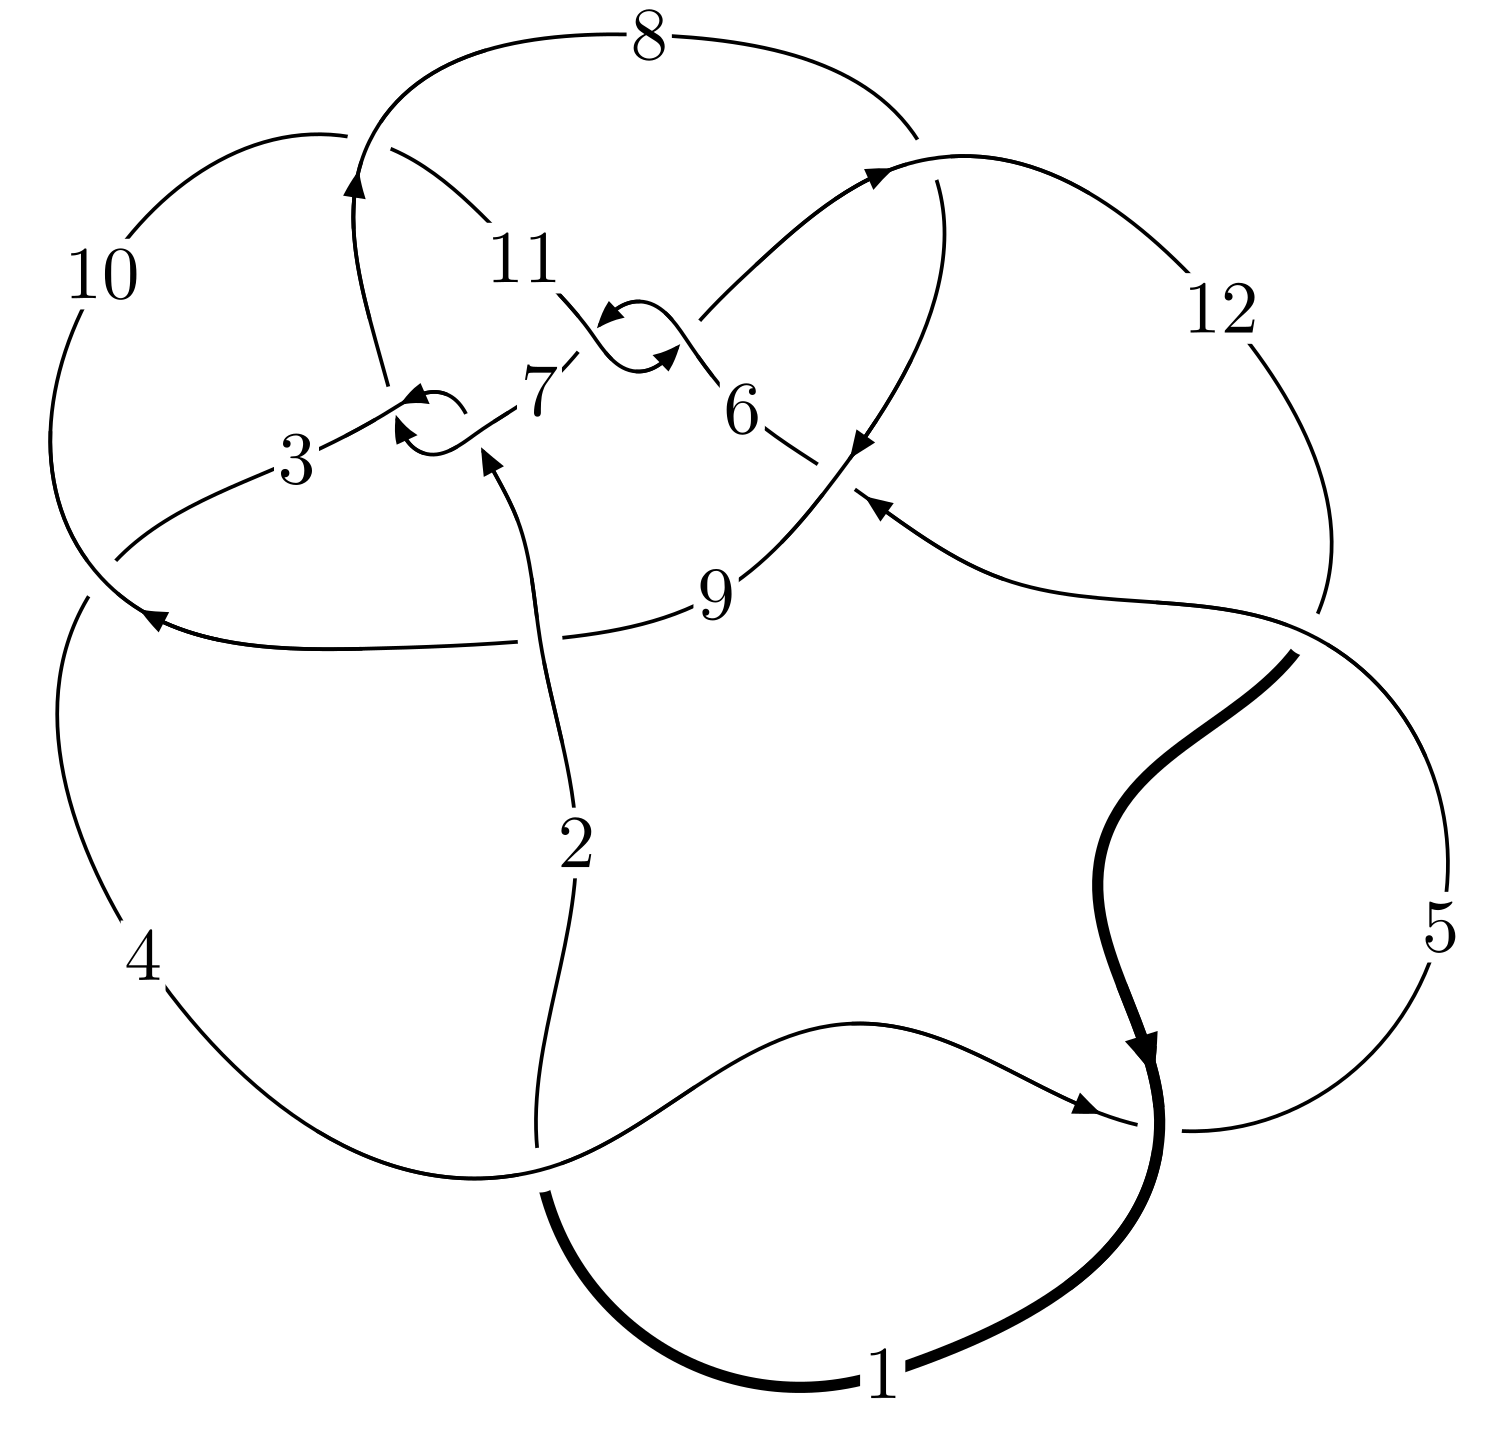
\includegraphics[width=112pt]{../../../GIT/diagram.site/Diagrams/png/1887_12a_1086.png}\\
\ \ \ A knot diagram\footnotemark}&
\allowdisplaybreaks
\textbf{Linearized knot diagam} \\
\cline{2-2}
 &
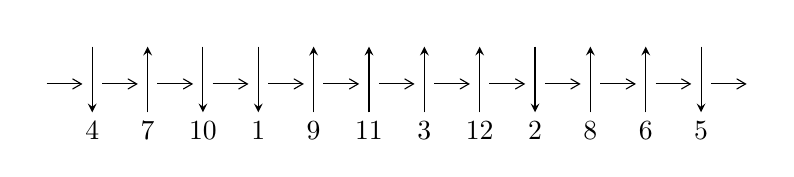
\begin{tikzpicture}[x=20pt, y=17pt]
	% nodes
	\node (C0) at (0, 0) {};
	\node (C1) at (1, 0) {};
	\node (C1U) at (1, +1) {};
	\node (C1D) at (1, -1) {4};

	\node (C2) at (2, 0) {};
	\node (C2U) at (2, +1) {};
	\node (C2D) at (2, -1) {7};

	\node (C3) at (3, 0) {};
	\node (C3U) at (3, +1) {};
	\node (C3D) at (3, -1) {10};

	\node (C4) at (4, 0) {};
	\node (C4U) at (4, +1) {};
	\node (C4D) at (4, -1) {1};

	\node (C5) at (5, 0) {};
	\node (C5U) at (5, +1) {};
	\node (C5D) at (5, -1) {9};

	\node (C6) at (6, 0) {};
	\node (C6U) at (6, +1) {};
	\node (C6D) at (6, -1) {11};

	\node (C7) at (7, 0) {};
	\node (C7U) at (7, +1) {};
	\node (C7D) at (7, -1) {3};

	\node (C8) at (8, 0) {};
	\node (C8U) at (8, +1) {};
	\node (C8D) at (8, -1) {12};

	\node (C9) at (9, 0) {};
	\node (C9U) at (9, +1) {};
	\node (C9D) at (9, -1) {2};

	\node (C10) at (10, 0) {};
	\node (C10U) at (10, +1) {};
	\node (C10D) at (10, -1) {8};

	\node (C11) at (11, 0) {};
	\node (C11U) at (11, +1) {};
	\node (C11D) at (11, -1) {6};

	\node (C12) at (12, 0) {};
	\node (C12U) at (12, +1) {};
	\node (C12D) at (12, -1) {5};
	\node (C13) at (13, 0) {};

	% arrows
	\draw[->,>={angle 60}]
	(C0) edge (C1) (C1) edge (C2) (C2) edge (C3) (C3) edge (C4) (C4) edge (C5) (C5) edge (C6) (C6) edge (C7) (C7) edge (C8) (C8) edge (C9) (C9) edge (C10) (C10) edge (C11) (C11) edge (C12) (C12) edge (C13) ;	\draw[->,>=stealth]
	(C1U) edge (C1D) (C2D) edge (C2U) (C3U) edge (C3D) (C4U) edge (C4D) (C5D) edge (C5U) (C6D) edge (C6U) (C7D) edge (C7U) (C8D) edge (C8U) (C9U) edge (C9D) (C10D) edge (C10U) (C11D) edge (C11U) (C12U) edge (C12D) ;
	\end{tikzpicture} \\
\hhline{~~} \\& 
\textbf{Solving Sequence} \\ \cline{2-2} 
 &
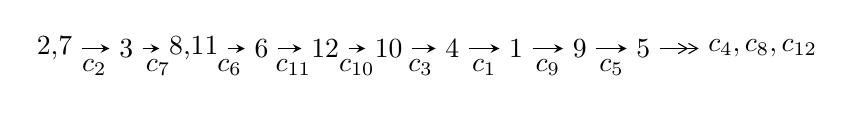
\begin{tikzpicture}[x=23pt, y=7pt]
	% node
	\node (A0) at (-1/8, 0) {2,7};
	\node (A1) at (1, 0) {3};
	\node (A2) at (33/16, 0) {8,11};
	\node (A3) at (25/8, 0) {6};
	\node (A4) at (33/8, 0) {12};
	\node (A5) at (41/8, 0) {10};
	\node (A6) at (49/8, 0) {4};
	\node (A7) at (57/8, 0) {1};
	\node (A8) at (65/8, 0) {9};
	\node (A9) at (73/8, 0) {5};
	\node (C1) at (1/2, -1) {$c_{2}$};
	\node (C2) at (3/2, -1) {$c_{7}$};
	\node (C3) at (21/8, -1) {$c_{6}$};
	\node (C4) at (29/8, -1) {$c_{11}$};
	\node (C5) at (37/8, -1) {$c_{10}$};
	\node (C6) at (45/8, -1) {$c_{3}$};
	\node (C7) at (53/8, -1) {$c_{1}$};
	\node (C8) at (61/8, -1) {$c_{9}$};
	\node (C9) at (69/8, -1) {$c_{5}$};
	\node (A10) at (11, 0) {$c_{4},c_{8},c_{12}$};

	% edge
	\draw[->,>=stealth]	
	(A0) edge (A1) (A1) edge (A2) (A2) edge (A3) (A3) edge (A4) (A4) edge (A5) (A5) edge (A6) (A6) edge (A7) (A7) edge (A8) (A8) edge (A9) ;
	\draw[->>,>={angle 60}]	
	(A9) edge (A10);
\end{tikzpicture} \\ 

\end{tabular} \\

\footnotetext{
The image of knot diagram is generated by the software ``\textbf{Draw programme}" developed by Andrew Bartholomew(\url{http://www.layer8.co.uk/maths/draw/index.htm\#Running-draw}), where we modified some parts for our purpose(\url{https://github.com/CATsTAILs/LinksPainter}).
}\phantom \\ \newline 
\centering \textbf{Ideals for irreducible components\footnotemark of $X_{\text{par}}$} 
 
\begin{align*}
I^u_{1}&=\langle 
7.29262\times10^{443} u^{125}-3.61065\times10^{443} u^{124}+\cdots+4.91844\times10^{444} b-2.41481\times10^{445},\\
\phantom{I^u_{1}}&\phantom{= \langle  }2.10816\times10^{445} u^{125}-1.92271\times10^{446} u^{124}+\cdots+2.30675\times10^{447} a+1.44340\times10^{449},\\
\phantom{I^u_{1}}&\phantom{= \langle  }u^{126}-35 u^{124}+\cdots-458 u+469\rangle \\
I^u_{2}&=\langle 
-296542176 u^{26}-86696195 u^{25}+\cdots+6531331 b-615569144,\\
\phantom{I^u_{2}}&\phantom{= \langle  }281791343 u^{26}+29749729 u^{25}+\cdots+6531331 a+697900612,\;u^{27}+u^{26}+\cdots-11 u^2+1\rangle \\
\\
\end{align*}
\raggedright * 2 irreducible components of $\dim_{\mathbb{C}}=0$, with total 153 representations.\\
\footnotetext{All coefficients of polynomials are rational numbers. But the coefficients are sometimes approximated in decimal forms when there is not enough margin.}
\newpage
\renewcommand{\arraystretch}{1}
\centering \section*{I. $I^u_{1}= \langle 7.29\times10^{443} u^{125}-3.61\times10^{443} u^{124}+\cdots+4.92\times10^{444} b-2.41\times10^{445},\;2.11\times10^{445} u^{125}-1.92\times10^{446} u^{124}+\cdots+2.31\times10^{447} a+1.44\times10^{449},\;u^{126}-35 u^{124}+\cdots-458 u+469 \rangle$}
\flushleft \textbf{(i) Arc colorings}\\
\begin{tabular}{m{7pt} m{180pt} m{7pt} m{180pt} }
\flushright $a_{2}=$&$\begin{pmatrix}1\\0\end{pmatrix}$ \\
\flushright $a_{7}=$&$\begin{pmatrix}0\\u\end{pmatrix}$ \\
\flushright $a_{3}=$&$\begin{pmatrix}1\\- u^2\end{pmatrix}$ \\
\flushright $a_{8}=$&$\begin{pmatrix}u\\- u^3+u\end{pmatrix}$ \\
\flushright $a_{11}=$&$\begin{pmatrix}-0.00913910 u^{125}+0.0833514 u^{124}+\cdots+86.9145 u-62.5728\\-0.148271 u^{125}+0.0734106 u^{124}+\cdots+45.8341 u+4.90970\end{pmatrix}$ \\
\flushright $a_{6}=$&$\begin{pmatrix}-0.173676 u^{125}+0.157828 u^{124}+\cdots+114.206 u-76.3215\\0.269095 u^{125}-0.211516 u^{124}+\cdots-279.017 u+118.949\end{pmatrix}$ \\
\flushright $a_{12}=$&$\begin{pmatrix}-0.119400 u^{125}-0.0244234 u^{124}+\cdots-84.3500 u+77.2817\\-0.0890187 u^{125}+0.0626953 u^{124}+\cdots+97.8027 u-54.2732\end{pmatrix}$ \\
\flushright $a_{10}=$&$\begin{pmatrix}0.126665 u^{125}+0.00735830 u^{124}+\cdots+25.1865 u-54.6294\\-0.145609 u^{125}+0.105822 u^{124}+\cdots+82.6032 u-22.7877\end{pmatrix}$ \\
\flushright $a_{4}=$&$\begin{pmatrix}-0.123590 u^{125}+0.0879692 u^{124}+\cdots+96.7714 u-28.0209\\-0.0488947 u^{125}+0.0609753 u^{124}+\cdots-37.4180 u+8.66197\end{pmatrix}$ \\
\flushright $a_{1}=$&$\begin{pmatrix}-0.654817 u^{125}+0.426479 u^{124}+\cdots+717.830 u-300.066\\0.0260049 u^{125}-0.0344322 u^{124}+\cdots-33.4096 u+18.5684\end{pmatrix}$ \\
\flushright $a_{9}=$&$\begin{pmatrix}-0.0189436 u^{125}+0.113181 u^{124}+\cdots+107.790 u-77.4171\\-0.145609 u^{125}+0.105822 u^{124}+\cdots+82.6032 u-22.7877\end{pmatrix}$ \\
\flushright $a_{5}=$&$\begin{pmatrix}-0.144394 u^{125}+0.183768 u^{124}+\cdots+161.092 u-116.204\\-0.159305 u^{125}+0.168067 u^{124}+\cdots+89.4490 u-53.8466\end{pmatrix}$\\&\end{tabular}
\flushleft \textbf{(ii) Obstruction class $= -1$}\\~\\
\flushleft \textbf{(iii) Cusp Shapes $= 0.0165479 u^{125}-0.311309 u^{124}+\cdots-172.863 u+172.842$}\\~\\
\newpage\renewcommand{\arraystretch}{1}
\flushleft \textbf{(iv) u-Polynomials at the component}\newline \\
\begin{tabular}{m{50pt}|m{274pt}}
Crossings & \hspace{64pt}u-Polynomials at each crossing \\
\hline $$\begin{aligned}c_{1},c_{4},c_{12}\end{aligned}$$&$\begin{aligned}
&u^{126}-5 u^{125}+\cdots+30 u-1
\end{aligned}$\\
\hline $$\begin{aligned}c_{2},c_{7}\end{aligned}$$&$\begin{aligned}
&u^{126}-35 u^{124}+\cdots-458 u+469
\end{aligned}$\\
\hline $$\begin{aligned}c_{3}\end{aligned}$$&$\begin{aligned}
&u^{126}+u^{125}+\cdots+1130931 u-66457
\end{aligned}$\\
\hline $$\begin{aligned}c_{5}\end{aligned}$$&$\begin{aligned}
&u^{126}-7 u^{125}+\cdots+106 u-7
\end{aligned}$\\
\hline $$\begin{aligned}c_{6},c_{11}\end{aligned}$$&$\begin{aligned}
&u^{126}- u^{125}+\cdots-68860 u-3292
\end{aligned}$\\
\hline $$\begin{aligned}c_{8}\end{aligned}$$&$\begin{aligned}
&u^{126}-9 u^{124}+\cdots+3761 u+521
\end{aligned}$\\
\hline $$\begin{aligned}c_{9}\end{aligned}$$&$\begin{aligned}
&u^{126}-3 u^{125}+\cdots+15229088 u-1636828
\end{aligned}$\\
\hline $$\begin{aligned}c_{10}\end{aligned}$$&$\begin{aligned}
&u^{126}-12 u^{125}+\cdots-1879129 u+1027873
\end{aligned}$\\
\hline
\end{tabular}\\~\\
\newpage\renewcommand{\arraystretch}{1}
\flushleft \textbf{(v) Riley Polynomials at the component}\newline \\
\begin{tabular}{m{50pt}|m{274pt}}
Crossings & \hspace{64pt}Riley Polynomials at each crossing \\
\hline $$\begin{aligned}c_{1},c_{4},c_{12}\end{aligned}$$&$\begin{aligned}
&y^{126}+137 y^{125}+\cdots-46 y+1
\end{aligned}$\\
\hline $$\begin{aligned}c_{2},c_{7}\end{aligned}$$&$\begin{aligned}
&y^{126}-70 y^{125}+\cdots-1412280 y+219961
\end{aligned}$\\
\hline $$\begin{aligned}c_{3}\end{aligned}$$&$\begin{aligned}
&y^{126}+51 y^{125}+\cdots+129805452721 y+4416532849
\end{aligned}$\\
\hline $$\begin{aligned}c_{5}\end{aligned}$$&$\begin{aligned}
&y^{126}-7 y^{125}+\cdots+5088 y+49
\end{aligned}$\\
\hline $$\begin{aligned}c_{6},c_{11}\end{aligned}$$&$\begin{aligned}
&y^{126}+93 y^{125}+\cdots-118823008 y+10837264
\end{aligned}$\\
\hline $$\begin{aligned}c_{8}\end{aligned}$$&$\begin{aligned}
&y^{126}-18 y^{125}+\cdots-15152735 y+271441
\end{aligned}$\\
\hline $$\begin{aligned}c_{9}\end{aligned}$$&$\begin{aligned}
&y^{126}+35 y^{125}+\cdots-24617509435312 y+2679205901584
\end{aligned}$\\
\hline $$\begin{aligned}c_{10}\end{aligned}$$&$\begin{aligned}
&y^{126}-14 y^{125}+\cdots-60668343049755 y+1056522904129
\end{aligned}$\\
\hline
\end{tabular}\\~\\
\newpage\flushleft \textbf{(vi) Complex Volumes and Cusp Shapes}
$$\begin{array}{c|c|c}  
\text{Solutions to }I^u_{1}& \I (\text{vol} + \sqrt{-1}CS) & \text{Cusp shape}\\
 \hline 
\begin{aligned}
u &= -0.970623 + 0.109965 I \\
a &= \phantom{-}0.36667 - 1.47144 I \\
b &= \phantom{-}1.76970 + 0.73739 I\end{aligned}
 & \phantom{-}7.09581 - 0.46489 I & \phantom{-0.000000 } 0 \\ \hline\begin{aligned}
u &= -0.970623 - 0.109965 I \\
a &= \phantom{-}0.36667 + 1.47144 I \\
b &= \phantom{-}1.76970 - 0.73739 I\end{aligned}
 & \phantom{-}7.09581 + 0.46489 I & \phantom{-0.000000 } 0 \\ \hline\begin{aligned}
u &= \phantom{-}0.942405 + 0.256456 I \\
a &= -0.96158 - 1.33084 I \\
b &= -1.57738 + 0.21976 I\end{aligned}
 & -1.55700 + 2.33827 I & \phantom{-0.000000 } 0 \\ \hline\begin{aligned}
u &= \phantom{-}0.942405 - 0.256456 I \\
a &= -0.96158 + 1.33084 I \\
b &= -1.57738 - 0.21976 I\end{aligned}
 & -1.55700 - 2.33827 I & \phantom{-0.000000 } 0 \\ \hline\begin{aligned}
u &= -0.966945 + 0.376641 I \\
a &= \phantom{-}1.000970 - 0.967740 I \\
b &= \phantom{-}1.71337 + 0.09779 I\end{aligned}
 & -2.75117 - 6.67930 I & \phantom{-0.000000 } 0 \\ \hline\begin{aligned}
u &= -0.966945 - 0.376641 I \\
a &= \phantom{-}1.000970 + 0.967740 I \\
b &= \phantom{-}1.71337 - 0.09779 I\end{aligned}
 & -2.75117 + 6.67930 I & \phantom{-0.000000 } 0 \\ \hline\begin{aligned}
u &= -0.857152 + 0.424347 I \\
a &= -0.517437 + 1.016120 I \\
b &= -2.03199 - 0.05964 I\end{aligned}
 & -3.04889 - 1.45471 I & \phantom{-0.000000 } 0 \\ \hline\begin{aligned}
u &= -0.857152 - 0.424347 I \\
a &= -0.517437 - 1.016120 I \\
b &= -2.03199 + 0.05964 I\end{aligned}
 & -3.04889 + 1.45471 I & \phantom{-0.000000 } 0 \\ \hline\begin{aligned}
u &= -0.908345 + 0.289800 I \\
a &= -0.241354 + 1.041250 I \\
b &= -2.21506 + 1.30506 I\end{aligned}
 & \phantom{-}4.19848 + 4.73980 I & \phantom{-0.000000 } 0 \\ \hline\begin{aligned}
u &= -0.908345 - 0.289800 I \\
a &= -0.241354 - 1.041250 I \\
b &= -2.21506 - 1.30506 I\end{aligned}
 & \phantom{-}4.19848 - 4.73980 I & \phantom{-0.000000 } 0\\
 \hline 
 \end{array}$$\newpage$$\begin{array}{c|c|c}  
\text{Solutions to }I^u_{1}& \I (\text{vol} + \sqrt{-1}CS) & \text{Cusp shape}\\
 \hline 
\begin{aligned}
u &= \phantom{-}0.092548 + 0.944929 I \\
a &= \phantom{-}0.021337 + 0.949815 I \\
b &= \phantom{-}0.490137 + 0.965918 I\end{aligned}
 & \phantom{-}0.62819 + 3.35726 I & \phantom{-0.000000 } 0 \\ \hline\begin{aligned}
u &= \phantom{-}0.092548 - 0.944929 I \\
a &= \phantom{-}0.021337 - 0.949815 I \\
b &= \phantom{-}0.490137 - 0.965918 I\end{aligned}
 & \phantom{-}0.62819 - 3.35726 I & \phantom{-0.000000 } 0 \\ \hline\begin{aligned}
u &= \phantom{-}0.010712 + 0.947670 I \\
a &= \phantom{-}0.012888 + 0.991675 I \\
b &= -0.271624 + 0.781462 I\end{aligned}
 & \phantom{-}8.18596 - 7.22783 I & \phantom{-0.000000 } 0 \\ \hline\begin{aligned}
u &= \phantom{-}0.010712 - 0.947670 I \\
a &= \phantom{-}0.012888 - 0.991675 I \\
b &= -0.271624 - 0.781462 I\end{aligned}
 & \phantom{-}8.18596 + 7.22783 I & \phantom{-0.000000 } 0 \\ \hline\begin{aligned}
u &= \phantom{-}0.882545 + 0.337456 I \\
a &= \phantom{-}0.339882 + 1.040700 I \\
b &= \phantom{-}2.20785 + 0.63143 I\end{aligned}
 & -2.67573 - 2.21056 I & \phantom{-0.000000 } 0 \\ \hline\begin{aligned}
u &= \phantom{-}0.882545 - 0.337456 I \\
a &= \phantom{-}0.339882 - 1.040700 I \\
b &= \phantom{-}2.20785 - 0.63143 I\end{aligned}
 & -2.67573 + 2.21056 I & \phantom{-0.000000 } 0 \\ \hline\begin{aligned}
u &= \phantom{-}0.617474 + 0.671103 I \\
a &= \phantom{-}0.94348 + 1.23326 I \\
b &= \phantom{-}2.56949 - 0.80314 I\end{aligned}
 & \phantom{-}4.05561 + 2.75690 I & \phantom{-0.000000 } 0 \\ \hline\begin{aligned}
u &= \phantom{-}0.617474 - 0.671103 I \\
a &= \phantom{-}0.94348 - 1.23326 I \\
b &= \phantom{-}2.56949 + 0.80314 I\end{aligned}
 & \phantom{-}4.05561 - 2.75690 I & \phantom{-0.000000 } 0 \\ \hline\begin{aligned}
u &= \phantom{-}0.218519 + 1.078790 I \\
a &= \phantom{-}1.077550 + 0.243009 I \\
b &= \phantom{-}1.59592 + 0.06226 I\end{aligned}
 & -0.10267 + 2.30053 I & \phantom{-0.000000 } 0 \\ \hline\begin{aligned}
u &= \phantom{-}0.218519 - 1.078790 I \\
a &= \phantom{-}1.077550 - 0.243009 I \\
b &= \phantom{-}1.59592 - 0.06226 I\end{aligned}
 & -0.10267 - 2.30053 I & \phantom{-0.000000 } 0\\
 \hline 
 \end{array}$$\newpage$$\begin{array}{c|c|c}  
\text{Solutions to }I^u_{1}& \I (\text{vol} + \sqrt{-1}CS) & \text{Cusp shape}\\
 \hline 
\begin{aligned}
u &= \phantom{-}0.999786 + 0.467391 I \\
a &= -0.972717 - 0.763915 I \\
b &= -1.80531 + 0.04063 I\end{aligned}
 & \phantom{-}3.05566 + 9.72046 I & \phantom{-0.000000 } 0 \\ \hline\begin{aligned}
u &= \phantom{-}0.999786 - 0.467391 I \\
a &= -0.972717 + 0.763915 I \\
b &= -1.80531 - 0.04063 I\end{aligned}
 & \phantom{-}3.05566 - 9.72046 I & \phantom{-0.000000 } 0 \\ \hline\begin{aligned}
u &= \phantom{-}0.675343 + 0.874019 I \\
a &= \phantom{-}1.041160 + 0.664860 I \\
b &= \phantom{-}1.60190 - 0.42948 I\end{aligned}
 & \phantom{-}1.65677 + 3.09355 I & \phantom{-0.000000 } 0 \\ \hline\begin{aligned}
u &= \phantom{-}0.675343 - 0.874019 I \\
a &= \phantom{-}1.041160 - 0.664860 I \\
b &= \phantom{-}1.60190 + 0.42948 I\end{aligned}
 & \phantom{-}1.65677 - 3.09355 I & \phantom{-0.000000 } 0 \\ \hline\begin{aligned}
u &= -0.871890 + 0.187558 I \\
a &= -0.43147 + 1.41778 I \\
b &= -0.38719 - 2.93184 I\end{aligned}
 & \phantom{-}3.86186 - 6.91825 I & \phantom{-0.000000 } 0 \\ \hline\begin{aligned}
u &= -0.871890 - 0.187558 I \\
a &= -0.43147 - 1.41778 I \\
b &= -0.38719 + 2.93184 I\end{aligned}
 & \phantom{-}3.86186 + 6.91825 I & \phantom{-0.000000 } 0 \\ \hline\begin{aligned}
u &= \phantom{-}0.940987 + 0.588632 I \\
a &= -0.580842 - 0.647536 I \\
b &= -2.56386 + 1.38056 I\end{aligned}
 & \phantom{-}9.05513 + 2.33946 I & \phantom{-0.000000 } 0 \\ \hline\begin{aligned}
u &= \phantom{-}0.940987 - 0.588632 I \\
a &= -0.580842 + 0.647536 I \\
b &= -2.56386 - 1.38056 I\end{aligned}
 & \phantom{-}9.05513 - 2.33946 I & \phantom{-0.000000 } 0 \\ \hline\begin{aligned}
u &= -0.523619 + 0.706080 I \\
a &= -1.26923 + 0.78134 I \\
b &= -1.36490 - 0.45951 I\end{aligned}
 & -3.46638 - 2.61366 I & \phantom{-0.000000 } 0 \\ \hline\begin{aligned}
u &= -0.523619 - 0.706080 I \\
a &= -1.26923 - 0.78134 I \\
b &= -1.36490 + 0.45951 I\end{aligned}
 & -3.46638 + 2.61366 I & \phantom{-0.000000 } 0\\
 \hline 
 \end{array}$$\newpage$$\begin{array}{c|c|c}  
\text{Solutions to }I^u_{1}& \I (\text{vol} + \sqrt{-1}CS) & \text{Cusp shape}\\
 \hline 
\begin{aligned}
u &= \phantom{-}0.874411\phantom{ +0.000000I} \\
a &= -1.57669\phantom{ +0.000000I} \\
b &= -1.03320\phantom{ +0.000000I}\end{aligned}
 & \phantom{-}1.00232\phantom{ +0.000000I} & \phantom{-0.000000 } 0 \\ \hline\begin{aligned}
u &= -0.782261 + 0.389760 I \\
a &= -0.929740 - 0.461657 I \\
b &= -0.319925 - 0.025276 I\end{aligned}
 & \phantom{-}5.84549 + 0.81290 I & \phantom{-0.000000 } 0 \\ \hline\begin{aligned}
u &= -0.782261 - 0.389760 I \\
a &= -0.929740 + 0.461657 I \\
b &= -0.319925 + 0.025276 I\end{aligned}
 & \phantom{-}5.84549 - 0.81290 I & \phantom{-0.000000 } 0 \\ \hline\begin{aligned}
u &= \phantom{-}1.064840 + 0.379693 I \\
a &= -0.413111 + 0.625058 I \\
b &= -0.667151 - 0.003480 I\end{aligned}
 & \phantom{-}3.51763 + 2.87060 I & \phantom{-0.000000 } 0 \\ \hline\begin{aligned}
u &= \phantom{-}1.064840 - 0.379693 I \\
a &= -0.413111 - 0.625058 I \\
b &= -0.667151 + 0.003480 I\end{aligned}
 & \phantom{-}3.51763 - 2.87060 I & \phantom{-0.000000 } 0 \\ \hline\begin{aligned}
u &= \phantom{-}0.695932 + 0.894230 I \\
a &= \phantom{-}0.284549 + 0.534176 I \\
b &= \phantom{-}1.134390 + 0.080449 I\end{aligned}
 & \phantom{-}1.15236 + 2.75670 I & \phantom{-0.000000 } 0 \\ \hline\begin{aligned}
u &= \phantom{-}0.695932 - 0.894230 I \\
a &= \phantom{-}0.284549 - 0.534176 I \\
b &= \phantom{-}1.134390 - 0.080449 I\end{aligned}
 & \phantom{-}1.15236 - 2.75670 I & \phantom{-0.000000 } 0 \\ \hline\begin{aligned}
u &= -1.119180 + 0.212654 I \\
a &= \phantom{-}0.588831 + 0.276461 I \\
b &= \phantom{-}0.916814 - 0.171103 I\end{aligned}
 & \phantom{-}4.74385 - 2.28444 I & \phantom{-0.000000 } 0 \\ \hline\begin{aligned}
u &= -1.119180 - 0.212654 I \\
a &= \phantom{-}0.588831 - 0.276461 I \\
b &= \phantom{-}0.916814 + 0.171103 I\end{aligned}
 & \phantom{-}4.74385 + 2.28444 I & \phantom{-0.000000 } 0 \\ \hline\begin{aligned}
u &= -0.258454 + 1.109840 I \\
a &= -1.044390 + 0.667910 I \\
b &= -2.10351 - 0.15975 I\end{aligned}
 & \phantom{-}3.95892 + 12.30210 I & \phantom{-0.000000 } 0\\
 \hline 
 \end{array}$$\newpage$$\begin{array}{c|c|c}  
\text{Solutions to }I^u_{1}& \I (\text{vol} + \sqrt{-1}CS) & \text{Cusp shape}\\
 \hline 
\begin{aligned}
u &= -0.258454 - 1.109840 I \\
a &= -1.044390 - 0.667910 I \\
b &= -2.10351 + 0.15975 I\end{aligned}
 & \phantom{-}3.95892 - 12.30210 I & \phantom{-0.000000 } 0 \\ \hline\begin{aligned}
u &= -0.719200 + 0.466600 I \\
a &= -0.95049 + 1.22827 I \\
b &= -1.49059 - 1.17047 I\end{aligned}
 & -3.53434 - 2.31998 I & \phantom{-0.000000 } 0 \\ \hline\begin{aligned}
u &= -0.719200 - 0.466600 I \\
a &= -0.95049 - 1.22827 I \\
b &= -1.49059 + 1.17047 I\end{aligned}
 & -3.53434 + 2.31998 I & \phantom{-0.000000 } 0 \\ \hline\begin{aligned}
u &= \phantom{-}0.311379 + 1.111650 I \\
a &= \phantom{-}0.978705 + 0.700895 I \\
b &= \phantom{-}2.13343 - 0.09626 I\end{aligned}
 & -3.24325 - 8.35925 I & \phantom{-0.000000 } 0 \\ \hline\begin{aligned}
u &= \phantom{-}0.311379 - 1.111650 I \\
a &= \phantom{-}0.978705 - 0.700895 I \\
b &= \phantom{-}2.13343 + 0.09626 I\end{aligned}
 & -3.24325 + 8.35925 I & \phantom{-0.000000 } 0 \\ \hline\begin{aligned}
u &= \phantom{-}1.008620 + 0.569134 I \\
a &= \phantom{-}0.693571 + 0.714935 I \\
b &= \phantom{-}1.48552 - 0.55280 I\end{aligned}
 & \phantom{-}2.19627 + 3.26013 I & \phantom{-0.000000 } 0 \\ \hline\begin{aligned}
u &= \phantom{-}1.008620 - 0.569134 I \\
a &= \phantom{-}0.693571 - 0.714935 I \\
b &= \phantom{-}1.48552 + 0.55280 I\end{aligned}
 & \phantom{-}2.19627 - 3.26013 I & \phantom{-0.000000 } 0 \\ \hline\begin{aligned}
u &= -1.073730 + 0.450599 I \\
a &= \phantom{-}0.356133 + 0.729758 I \\
b &= \phantom{-}0.648328 + 0.072797 I\end{aligned}
 & \phantom{-}9.49428 - 3.56556 I & \phantom{-0.000000 } 0 \\ \hline\begin{aligned}
u &= -1.073730 - 0.450599 I \\
a &= \phantom{-}0.356133 - 0.729758 I \\
b &= \phantom{-}0.648328 - 0.072797 I\end{aligned}
 & \phantom{-}9.49428 + 3.56556 I & \phantom{-0.000000 } 0 \\ \hline\begin{aligned}
u &= \phantom{-}0.797029 + 0.238822 I \\
a &= \phantom{-}0.60456 + 1.49514 I \\
b &= \phantom{-}0.70268 - 2.17049 I\end{aligned}
 & -3.12454 + 4.92510 I & \phantom{-0.000000 } 0\\
 \hline 
 \end{array}$$\newpage$$\begin{array}{c|c|c}  
\text{Solutions to }I^u_{1}& \I (\text{vol} + \sqrt{-1}CS) & \text{Cusp shape}\\
 \hline 
\begin{aligned}
u &= \phantom{-}0.797029 - 0.238822 I \\
a &= \phantom{-}0.60456 - 1.49514 I \\
b &= \phantom{-}0.70268 + 2.17049 I\end{aligned}
 & -3.12454 - 4.92510 I & \phantom{-0.000000 } 0 \\ \hline\begin{aligned}
u &= -0.394117 + 1.111950 I \\
a &= -0.853379 + 0.777888 I \\
b &= -2.20792 + 0.06848 I\end{aligned}
 & -3.78607 + 2.75727 I & \phantom{-0.000000 } 0 \\ \hline\begin{aligned}
u &= -0.394117 - 1.111950 I \\
a &= -0.853379 - 0.777888 I \\
b &= -2.20792 - 0.06848 I\end{aligned}
 & -3.78607 - 2.75727 I & \phantom{-0.000000 } 0 \\ \hline\begin{aligned}
u &= \phantom{-}0.792927 + 0.198436 I \\
a &= -0.24880 - 1.94336 I \\
b &= -0.860975 + 0.809139 I\end{aligned}
 & -2.15309 - 0.12831 I & \phantom{-0.000000 } 0 \\ \hline\begin{aligned}
u &= \phantom{-}0.792927 - 0.198436 I \\
a &= -0.24880 + 1.94336 I \\
b &= -0.860975 - 0.809139 I\end{aligned}
 & -2.15309 + 0.12831 I & \phantom{-0.000000 } 0 \\ \hline\begin{aligned}
u &= -0.781562 + 0.186528 I \\
a &= \phantom{-}1.10944 + 0.92626 I \\
b &= \phantom{-}0.946496 + 0.148654 I\end{aligned}
 & \phantom{-}5.50194 - 3.75805 I & \phantom{-0.000000 -}0. + 7.30757 I \\ \hline\begin{aligned}
u &= -0.781562 - 0.186528 I \\
a &= \phantom{-}1.10944 - 0.92626 I \\
b &= \phantom{-}0.946496 - 0.148654 I\end{aligned}
 & \phantom{-}5.50194 + 3.75805 I & \phantom{-0.000000 } 0. - 7.30757 I \\ \hline\begin{aligned}
u &= -1.143410 + 0.368152 I \\
a &= \phantom{-}0.084839 + 0.695642 I \\
b &= \phantom{-}0.292187 + 0.317180 I\end{aligned}
 & \phantom{-}9.32845 - 0.15577 I & \phantom{-0.000000 } 0 \\ \hline\begin{aligned}
u &= -1.143410 - 0.368152 I \\
a &= \phantom{-}0.084839 - 0.695642 I \\
b &= \phantom{-}0.292187 - 0.317180 I\end{aligned}
 & \phantom{-}9.32845 + 0.15577 I & \phantom{-0.000000 } 0 \\ \hline\begin{aligned}
u &= \phantom{-}1.189610 + 0.190263 I \\
a &= \phantom{-}0.689839 - 0.825068 I \\
b &= -0.208873 + 0.261682 I\end{aligned}
 & \phantom{-}2.55795 + 0.40515 I & \phantom{-0.000000 } 0\\
 \hline 
 \end{array}$$\newpage$$\begin{array}{c|c|c}  
\text{Solutions to }I^u_{1}& \I (\text{vol} + \sqrt{-1}CS) & \text{Cusp shape}\\
 \hline 
\begin{aligned}
u &= \phantom{-}1.189610 - 0.190263 I \\
a &= \phantom{-}0.689839 + 0.825068 I \\
b &= -0.208873 - 0.261682 I\end{aligned}
 & \phantom{-}2.55795 - 0.40515 I & \phantom{-0.000000 } 0 \\ \hline\begin{aligned}
u &= -1.171720 + 0.297261 I \\
a &= -0.501837 - 1.292290 I \\
b &= \phantom{-}0.541604 + 0.368665 I\end{aligned}
 & \phantom{-}8.53747 - 5.00328 I & \phantom{-0.000000 } 0 \\ \hline\begin{aligned}
u &= -1.171720 - 0.297261 I \\
a &= -0.501837 + 1.292290 I \\
b &= \phantom{-}0.541604 - 0.368665 I\end{aligned}
 & \phantom{-}8.53747 + 5.00328 I & \phantom{-0.000000 } 0 \\ \hline\begin{aligned}
u &= \phantom{-}1.149020 + 0.400504 I \\
a &= -0.044347 + 0.511764 I \\
b &= -0.106887 - 0.111151 I\end{aligned}
 & \phantom{-}2.52008 + 1.33074 I & \phantom{-0.000000 } 0 \\ \hline\begin{aligned}
u &= \phantom{-}1.149020 - 0.400504 I \\
a &= -0.044347 - 0.511764 I \\
b &= -0.106887 + 0.111151 I\end{aligned}
 & \phantom{-}2.52008 - 1.33074 I & \phantom{-0.000000 } 0 \\ \hline\begin{aligned}
u &= -0.138999 + 0.759366 I \\
a &= \phantom{-}1.312110 - 0.461227 I \\
b &= \phantom{-}1.001010 + 0.503429 I\end{aligned}
 & -1.25264 + 2.36149 I & \phantom{-}3.02337 - 5.11352 I \\ \hline\begin{aligned}
u &= -0.138999 - 0.759366 I \\
a &= \phantom{-}1.312110 + 0.461227 I \\
b &= \phantom{-}1.001010 - 0.503429 I\end{aligned}
 & -1.25264 - 2.36149 I & \phantom{-}3.02337 + 5.11352 I \\ \hline\begin{aligned}
u &= \phantom{-}1.217620 + 0.167615 I \\
a &= -0.569466 + 0.104589 I \\
b &= -1.103690 - 0.232877 I\end{aligned}
 & \phantom{-}11.79450 + 2.63794 I & \phantom{-0.000000 } 0 \\ \hline\begin{aligned}
u &= \phantom{-}1.217620 - 0.167615 I \\
a &= -0.569466 - 0.104589 I \\
b &= -1.103690 + 0.232877 I\end{aligned}
 & \phantom{-}11.79450 - 2.63794 I & \phantom{-0.000000 } 0 \\ \hline\begin{aligned}
u &= \phantom{-}0.300849 + 1.192090 I \\
a &= -0.836379 - 0.186369 I \\
b &= -1.74416 + 0.66811 I\end{aligned}
 & -3.64149 + 0.33300 I & \phantom{-0.000000 } 0\\
 \hline 
 \end{array}$$\newpage$$\begin{array}{c|c|c}  
\text{Solutions to }I^u_{1}& \I (\text{vol} + \sqrt{-1}CS) & \text{Cusp shape}\\
 \hline 
\begin{aligned}
u &= \phantom{-}0.300849 - 1.192090 I \\
a &= -0.836379 + 0.186369 I \\
b &= -1.74416 - 0.66811 I\end{aligned}
 & -3.64149 - 0.33300 I & \phantom{-0.000000 } 0 \\ \hline\begin{aligned}
u &= \phantom{-}0.165351 + 0.728645 I \\
a &= -1.097140 - 0.705621 I \\
b &= -0.704111 + 0.585780 I\end{aligned}
 & \phantom{-}5.54492 - 3.39623 I & \phantom{-}4.79113 + 3.93438 I \\ \hline\begin{aligned}
u &= \phantom{-}0.165351 - 0.728645 I \\
a &= -1.097140 + 0.705621 I \\
b &= -0.704111 - 0.585780 I\end{aligned}
 & \phantom{-}5.54492 + 3.39623 I & \phantom{-}4.79113 - 3.93438 I \\ \hline\begin{aligned}
u &= \phantom{-}0.492316 + 0.552431 I \\
a &= -0.96762 - 1.61134 I \\
b &= -0.641552 + 0.503324 I\end{aligned}
 & \phantom{-}1.55800 - 5.60766 I & \phantom{-}1.12260 + 2.03980 I \\ \hline\begin{aligned}
u &= \phantom{-}0.492316 - 0.552431 I \\
a &= -0.96762 + 1.61134 I \\
b &= -0.641552 - 0.503324 I\end{aligned}
 & \phantom{-}1.55800 + 5.60766 I & \phantom{-}1.12260 - 2.03980 I \\ \hline\begin{aligned}
u &= \phantom{-}1.159920 + 0.503454 I \\
a &= -0.616467 - 0.571341 I \\
b &= -2.26723 + 0.12128 I\end{aligned}
 & \phantom{-}8.41120 + 8.01034 I & \phantom{-0.000000 } 0 \\ \hline\begin{aligned}
u &= \phantom{-}1.159920 - 0.503454 I \\
a &= -0.616467 + 0.571341 I \\
b &= -2.26723 - 0.12128 I\end{aligned}
 & \phantom{-}8.41120 - 8.01034 I & \phantom{-0.000000 } 0 \\ \hline\begin{aligned}
u &= -1.212680 + 0.371564 I \\
a &= \phantom{-}0.078212 + 0.267912 I \\
b &= \phantom{-}0.291183 - 0.611037 I\end{aligned}
 & \phantom{-}2.06132 - 4.33077 I & \phantom{-0.000000 } 0 \\ \hline\begin{aligned}
u &= -1.212680 - 0.371564 I \\
a &= \phantom{-}0.078212 - 0.267912 I \\
b &= \phantom{-}0.291183 + 0.611037 I\end{aligned}
 & \phantom{-}2.06132 + 4.33077 I & \phantom{-0.000000 } 0 \\ \hline\begin{aligned}
u &= -1.174140 + 0.498983 I \\
a &= \phantom{-}0.609389 - 0.649320 I \\
b &= \phantom{-}2.11404 + 0.29591 I\end{aligned}
 & \phantom{-}1.75505 - 7.01207 I & \phantom{-0.000000 } 0\\
 \hline 
 \end{array}$$\newpage$$\begin{array}{c|c|c}  
\text{Solutions to }I^u_{1}& \I (\text{vol} + \sqrt{-1}CS) & \text{Cusp shape}\\
 \hline 
\begin{aligned}
u &= -1.174140 - 0.498983 I \\
a &= \phantom{-}0.609389 + 0.649320 I \\
b &= \phantom{-}2.11404 - 0.29591 I\end{aligned}
 & \phantom{-}1.75505 + 7.01207 I & \phantom{-0.000000 } 0 \\ \hline\begin{aligned}
u &= \phantom{-}1.241500 + 0.339354 I \\
a &= -0.118974 + 0.101131 I \\
b &= -0.526832 - 0.911895 I\end{aligned}
 & \phantom{-}8.32979 + 6.48068 I & \phantom{-0.000000 } 0 \\ \hline\begin{aligned}
u &= \phantom{-}1.241500 - 0.339354 I \\
a &= -0.118974 - 0.101131 I \\
b &= -0.526832 + 0.911895 I\end{aligned}
 & \phantom{-}8.32979 - 6.48068 I & \phantom{-0.000000 } 0 \\ \hline\begin{aligned}
u &= -1.084230 + 0.744299 I \\
a &= \phantom{-}0.547218 - 0.574475 I \\
b &= \phantom{-}2.16145 + 1.04357 I\end{aligned}
 & \phantom{-}1.30001 - 3.27173 I & \phantom{-0.000000 } 0 \\ \hline\begin{aligned}
u &= -1.084230 - 0.744299 I \\
a &= \phantom{-}0.547218 + 0.574475 I \\
b &= \phantom{-}2.16145 - 1.04357 I\end{aligned}
 & \phantom{-}1.30001 + 3.27173 I & \phantom{-0.000000 } 0 \\ \hline\begin{aligned}
u &= \phantom{-}1.270760 + 0.391807 I \\
a &= -0.521070 - 0.795438 I \\
b &= -1.80150 + 0.36154 I\end{aligned}
 & \phantom{-}1.49681 + 6.23106 I & \phantom{-0.000000 } 0 \\ \hline\begin{aligned}
u &= \phantom{-}1.270760 - 0.391807 I \\
a &= -0.521070 + 0.795438 I \\
b &= -1.80150 - 0.36154 I\end{aligned}
 & \phantom{-}1.49681 - 6.23106 I & \phantom{-0.000000 } 0 \\ \hline\begin{aligned}
u &= \phantom{-}0.652264\phantom{ +0.000000I} \\
a &= \phantom{-}1.03101\phantom{ +0.000000I} \\
b &= \phantom{-}0.281959\phantom{ +0.000000I}\end{aligned}
 & \phantom{-}1.20245\phantom{ +0.000000I} & \phantom{-}10.9940\phantom{ +0.000000I} \\ \hline\begin{aligned}
u &= -1.275040 + 0.456056 I \\
a &= -0.941604 - 0.198837 I \\
b &= -0.263074 - 0.821531 I\end{aligned}
 & \phantom{-}4.76593 - 8.17743 I & \phantom{-0.000000 } 0 \\ \hline\begin{aligned}
u &= -1.275040 - 0.456056 I \\
a &= -0.941604 + 0.198837 I \\
b &= -0.263074 + 0.821531 I\end{aligned}
 & \phantom{-}4.76593 + 8.17743 I & \phantom{-0.000000 } 0\\
 \hline 
 \end{array}$$\newpage$$\begin{array}{c|c|c}  
\text{Solutions to }I^u_{1}& \I (\text{vol} + \sqrt{-1}CS) & \text{Cusp shape}\\
 \hline 
\begin{aligned}
u &= -0.292246 + 0.575557 I \\
a &= -0.917370 - 0.714132 I \\
b &= -0.371520 + 0.235817 I\end{aligned}
 & \phantom{-}7.30107 - 0.46604 I & \phantom{-}6.73871 + 1.91848 I \\ \hline\begin{aligned}
u &= -0.292246 - 0.575557 I \\
a &= -0.917370 + 0.714132 I \\
b &= -0.371520 - 0.235817 I\end{aligned}
 & \phantom{-}7.30107 + 0.46604 I & \phantom{-}6.73871 - 1.91848 I \\ \hline\begin{aligned}
u &= -0.543087 + 0.333468 I \\
a &= \phantom{-}0.72839 - 2.13501 I \\
b &= \phantom{-}0.558413 + 0.604662 I\end{aligned}
 & -4.01535 + 3.41959 I & -2.30368 + 0.21144 I \\ \hline\begin{aligned}
u &= -0.543087 - 0.333468 I \\
a &= \phantom{-}0.72839 + 2.13501 I \\
b &= \phantom{-}0.558413 - 0.604662 I\end{aligned}
 & -4.01535 - 3.41959 I & -2.30368 - 0.21144 I \\ \hline\begin{aligned}
u &= \phantom{-}1.274810 + 0.491288 I \\
a &= \phantom{-}0.864555 - 0.230360 I \\
b &= \phantom{-}0.399460 - 0.761795 I\end{aligned}
 & \phantom{-}12.0565 + 12.3113 I & \phantom{-0.000000 } 0 \\ \hline\begin{aligned}
u &= \phantom{-}1.274810 - 0.491288 I \\
a &= \phantom{-}0.864555 + 0.230360 I \\
b &= \phantom{-}0.399460 + 0.761795 I\end{aligned}
 & \phantom{-}12.0565 - 12.3113 I & \phantom{-0.000000 } 0 \\ \hline\begin{aligned}
u &= -1.361730 + 0.113588 I \\
a &= -0.385697 - 0.716871 I \\
b &= \phantom{-}0.129086 + 0.630162 I\end{aligned}
 & \phantom{-}3.29705 + 4.11928 I & \phantom{-0.000000 } 0 \\ \hline\begin{aligned}
u &= -1.361730 - 0.113588 I \\
a &= -0.385697 + 0.716871 I \\
b &= \phantom{-}0.129086 - 0.630162 I\end{aligned}
 & \phantom{-}3.29705 - 4.11928 I & \phantom{-0.000000 } 0 \\ \hline\begin{aligned}
u &= -1.339720 + 0.301551 I \\
a &= \phantom{-}0.442442 - 0.841602 I \\
b &= \phantom{-}1.67849 + 0.32054 I\end{aligned}
 & \phantom{-}7.97095 - 6.50583 I & \phantom{-0.000000 } 0 \\ \hline\begin{aligned}
u &= -1.339720 - 0.301551 I \\
a &= \phantom{-}0.442442 + 0.841602 I \\
b &= \phantom{-}1.67849 - 0.32054 I\end{aligned}
 & \phantom{-}7.97095 + 6.50583 I & \phantom{-0.000000 } 0\\
 \hline 
 \end{array}$$\newpage$$\begin{array}{c|c|c}  
\text{Solutions to }I^u_{1}& \I (\text{vol} + \sqrt{-1}CS) & \text{Cusp shape}\\
 \hline 
\begin{aligned}
u &= -1.321170 + 0.454924 I \\
a &= -0.733337 + 0.018294 I \\
b &= -0.536120 - 1.077190 I\end{aligned}
 & \phantom{-}12.34460 + 2.14848 I & \phantom{-0.000000 } 0 \\ \hline\begin{aligned}
u &= -1.321170 - 0.454924 I \\
a &= -0.733337 - 0.018294 I \\
b &= -0.536120 + 1.077190 I\end{aligned}
 & \phantom{-}12.34460 - 2.14848 I & \phantom{-0.000000 } 0 \\ \hline\begin{aligned}
u &= \phantom{-}1.326030 + 0.458330 I \\
a &= \phantom{-}0.972372 + 0.065808 I \\
b &= \phantom{-}0.327609 - 1.238650 I\end{aligned}
 & \phantom{-}4.63085 + 2.01487 I & \phantom{-0.000000 } 0 \\ \hline\begin{aligned}
u &= \phantom{-}1.326030 - 0.458330 I \\
a &= \phantom{-}0.972372 - 0.065808 I \\
b &= \phantom{-}0.327609 + 1.238650 I\end{aligned}
 & \phantom{-}4.63085 - 2.01487 I & \phantom{-0.000000 } 0 \\ \hline\begin{aligned}
u &= -1.255250 + 0.645885 I \\
a &= -0.858593 + 0.715882 I \\
b &= -2.09645 - 1.45278 I\end{aligned}
 & -0.92940 - 9.04679 I & \phantom{-0.000000 } 0 \\ \hline\begin{aligned}
u &= -1.255250 - 0.645885 I \\
a &= -0.858593 - 0.715882 I \\
b &= -2.09645 + 1.45278 I\end{aligned}
 & -0.92940 + 9.04679 I & \phantom{-0.000000 } 0 \\ \hline\begin{aligned}
u &= \phantom{-}1.26771 + 0.64097 I \\
a &= \phantom{-}0.814774 + 0.723594 I \\
b &= \phantom{-}2.23099 - 1.29420 I\end{aligned}
 & -0.1859 + 14.5941 I & \phantom{-0.000000 } 0 \\ \hline\begin{aligned}
u &= \phantom{-}1.26771 - 0.64097 I \\
a &= \phantom{-}0.814774 - 0.723594 I \\
b &= \phantom{-}2.23099 + 1.29420 I\end{aligned}
 & -0.1859 - 14.5941 I & \phantom{-0.000000 } 0 \\ \hline\begin{aligned}
u &= -1.28092 + 0.63273 I \\
a &= -0.791136 + 0.729120 I \\
b &= -2.32305 - 1.22310 I\end{aligned}
 & \phantom{-}7.1819 - 18.4916 I & \phantom{-0.000000 } 0 \\ \hline\begin{aligned}
u &= -1.28092 - 0.63273 I \\
a &= -0.791136 - 0.729120 I \\
b &= -2.32305 + 1.22310 I\end{aligned}
 & \phantom{-}7.1819 + 18.4916 I & \phantom{-0.000000 } 0\\
 \hline 
 \end{array}$$\newpage$$\begin{array}{c|c|c}  
\text{Solutions to }I^u_{1}& \I (\text{vol} + \sqrt{-1}CS) & \text{Cusp shape}\\
 \hline 
\begin{aligned}
u &= \phantom{-}1.24104 + 0.75808 I \\
a &= \phantom{-}1.051530 + 0.875991 I \\
b &= \phantom{-}2.52316 - 2.32345 I\end{aligned}
 & \phantom{-}5.34160 + 3.32403 I & \phantom{-0.000000 } 0 \\ \hline\begin{aligned}
u &= \phantom{-}1.24104 - 0.75808 I \\
a &= \phantom{-}1.051530 - 0.875991 I \\
b &= \phantom{-}2.52316 + 2.32345 I\end{aligned}
 & \phantom{-}5.34160 - 3.32403 I & \phantom{-0.000000 } 0 \\ \hline\begin{aligned}
u &= \phantom{-}1.30681 + 0.67419 I \\
a &= -0.471067 - 0.616995 I \\
b &= -1.92205 + 0.81411 I\end{aligned}
 & -0.36548 + 6.26801 I & \phantom{-0.000000 } 0 \\ \hline\begin{aligned}
u &= \phantom{-}1.30681 - 0.67419 I \\
a &= -0.471067 + 0.616995 I \\
b &= -1.92205 - 0.81411 I\end{aligned}
 & -0.36548 - 6.26801 I & \phantom{-0.000000 } 0 \\ \hline\begin{aligned}
u &= -0.78348 + 1.24630 I \\
a &= \phantom{-}0.619511 - 0.336925 I \\
b &= \phantom{-}1.99279 + 1.01793 I\end{aligned}
 & \phantom{-}0.25002 - 3.81753 I & \phantom{-0.000000 } 0 \\ \hline\begin{aligned}
u &= -0.78348 - 1.24630 I \\
a &= \phantom{-}0.619511 + 0.336925 I \\
b &= \phantom{-}1.99279 - 1.01793 I\end{aligned}
 & \phantom{-}0.25002 + 3.81753 I & \phantom{-0.000000 } 0 \\ \hline\begin{aligned}
u &= -0.131389 + 0.501912 I \\
a &= \phantom{-}0.463018 + 0.506197 I \\
b &= -0.420529 + 0.601464 I\end{aligned}
 & -1.13493 + 0.94147 I & -4.21874 - 2.34500 I \\ \hline\begin{aligned}
u &= -0.131389 - 0.501912 I \\
a &= \phantom{-}0.463018 - 0.506197 I \\
b &= -0.420529 - 0.601464 I\end{aligned}
 & -1.13493 - 0.94147 I & -4.21874 + 2.34500 I \\ \hline\begin{aligned}
u &= \phantom{-}1.46722 + 0.20354 I \\
a &= \phantom{-}0.255174 - 0.756956 I \\
b &= -0.275869 + 0.759974 I\end{aligned}
 & \phantom{-}10.15790 - 7.45001 I & \phantom{-0.000000 } 0 \\ \hline\begin{aligned}
u &= \phantom{-}1.46722 - 0.20354 I \\
a &= \phantom{-}0.255174 + 0.756956 I \\
b &= -0.275869 - 0.759974 I\end{aligned}
 & \phantom{-}10.15790 + 7.45001 I & \phantom{-0.000000 } 0\\
 \hline 
 \end{array}$$\newpage$$\begin{array}{c|c|c}  
\text{Solutions to }I^u_{1}& \I (\text{vol} + \sqrt{-1}CS) & \text{Cusp shape}\\
 \hline 
\begin{aligned}
u &= -1.44185 + 0.59051 I \\
a &= \phantom{-}0.413659 - 0.665951 I \\
b &= \phantom{-}1.70652 + 0.73088 I\end{aligned}
 & \phantom{-}4.95027 - 8.38558 I & \phantom{-0.000000 } 0 \\ \hline\begin{aligned}
u &= -1.44185 - 0.59051 I \\
a &= \phantom{-}0.413659 + 0.665951 I \\
b &= \phantom{-}1.70652 - 0.73088 I\end{aligned}
 & \phantom{-}4.95027 + 8.38558 I & \phantom{-0.000000 } 0 \\ \hline\begin{aligned}
u &= \phantom{-}0.195119 + 0.364133 I \\
a &= \phantom{-}0.971260 - 1.008830 I \\
b &= \phantom{-}0.199389 + 0.215350 I\end{aligned}
 & \phantom{-}1.319960 + 0.350002 I & \phantom{-}7.97653 - 0.58766 I \\ \hline\begin{aligned}
u &= \phantom{-}0.195119 - 0.364133 I \\
a &= \phantom{-}0.971260 + 1.008830 I \\
b &= \phantom{-}0.199389 - 0.215350 I\end{aligned}
 & \phantom{-}1.319960 - 0.350002 I & \phantom{-}7.97653 + 0.58766 I \\ \hline\begin{aligned}
u &= \phantom{-}0.098074 + 0.341468 I \\
a &= -1.85528 + 0.39319 I \\
b &= \phantom{-}0.493075 + 1.077430 I\end{aligned}
 & \phantom{-}4.88741 - 3.42237 I & \phantom{-}1.82670 + 2.65734 I \\ \hline\begin{aligned}
u &= \phantom{-}0.098074 - 0.341468 I \\
a &= -1.85528 - 0.39319 I \\
b &= \phantom{-}0.493075 - 1.077430 I\end{aligned}
 & \phantom{-}4.88741 + 3.42237 I & \phantom{-}1.82670 - 2.65734 I\\
 \hline 
 \end{array}$$\newpage\newpage\renewcommand{\arraystretch}{1}
\centering \section*{II. $I^u_{2}= \langle -2.97\times10^{8} u^{26}-8.67\times10^{7} u^{25}+\cdots+6.53\times10^{6} b-6.16\times10^{8},\;2.82\times10^{8} u^{26}+2.97\times10^{7} u^{25}+\cdots+6.53\times10^{6} a+6.98\times10^{8},\;u^{27}+u^{26}+\cdots-11 u^2+1 \rangle$}
\flushleft \textbf{(i) Arc colorings}\\
\begin{tabular}{m{7pt} m{180pt} m{7pt} m{180pt} }
\flushright $a_{2}=$&$\begin{pmatrix}1\\0\end{pmatrix}$ \\
\flushright $a_{7}=$&$\begin{pmatrix}0\\u\end{pmatrix}$ \\
\flushright $a_{3}=$&$\begin{pmatrix}1\\- u^2\end{pmatrix}$ \\
\flushright $a_{8}=$&$\begin{pmatrix}u\\- u^3+u\end{pmatrix}$ \\
\flushright $a_{11}=$&$\begin{pmatrix}-43.1446 u^{26}-4.55493 u^{25}+\cdots+102.918 u-106.854\\45.4030 u^{26}+13.2739 u^{25}+\cdots-113.510 u+94.2487\end{pmatrix}$ \\
\flushright $a_{6}=$&$\begin{pmatrix}47.8248 u^{26}+11.8549 u^{25}+\cdots-86.5156 u+82.6503\\-18.7731 u^{26}-15.4500 u^{25}+\cdots+20.9914 u+5.23085\end{pmatrix}$ \\
\flushright $a_{12}=$&$\begin{pmatrix}-25.5393 u^{26}-10.8391 u^{25}+\cdots+37.5220 u-9.95058\\-15.9395 u^{26}+0.796616 u^{25}+\cdots+45.6064 u-44.5238\end{pmatrix}$ \\
\flushright $a_{10}=$&$\begin{pmatrix}-71.3659 u^{26}-13.7069 u^{25}+\cdots+174.284 u-163.513\\28.2213 u^{26}+9.15194 u^{25}+\cdots-70.3659 u+56.6590\end{pmatrix}$ \\
\flushright $a_{4}=$&$\begin{pmatrix}91.3252 u^{26}+45.1086 u^{25}+\cdots-254.838 u+118.583\\-26.6662 u^{26}-8.67088 u^{25}+\cdots+83.3252 u-46.2166\end{pmatrix}$ \\
\flushright $a_{1}=$&$\begin{pmatrix}66.4791 u^{26}+6.15932 u^{25}+\cdots-155.922 u+137.571\\-20.6035 u^{26}-9.70298 u^{25}+\cdots+26.1497 u-17.9912\end{pmatrix}$ \\
\flushright $a_{9}=$&$\begin{pmatrix}-43.1446 u^{26}-4.55493 u^{25}+\cdots+103.918 u-106.854\\28.2213 u^{26}+9.15194 u^{25}+\cdots-70.3659 u+56.6590\end{pmatrix}$ \\
\flushright $a_{5}=$&$\begin{pmatrix}-15.7937 u^{26}+6.39736 u^{25}+\cdots+74.3803 u-94.9944\\52.4256 u^{26}+15.2951 u^{25}+\cdots-132.016 u+92.8970\end{pmatrix}$\\&\end{tabular}
\flushleft \textbf{(ii) Obstruction class $= 1$}\\~\\
\flushleft \textbf{(iii) Cusp Shapes $= -\frac{1237736833}{6531331} u^{26}-\frac{715022714}{6531331} u^{25}+\cdots+\frac{3021932240}{6531331} u-\frac{1104068601}{6531331}$}\\~\\
\newpage\renewcommand{\arraystretch}{1}
\flushleft \textbf{(iv) u-Polynomials at the component}\newline \\
\begin{tabular}{m{50pt}|m{274pt}}
Crossings & \hspace{64pt}u-Polynomials at each crossing \\
\hline $$\begin{aligned}c_{1},c_{12}\end{aligned}$$&$\begin{aligned}
&u^{27}-2 u^{26}+\cdots+2 u^2-1
\end{aligned}$\\
\hline $$\begin{aligned}c_{2}\end{aligned}$$&$\begin{aligned}
&u^{27}+u^{26}+\cdots-11 u^2+1
\end{aligned}$\\
\hline $$\begin{aligned}c_{3}\end{aligned}$$&$\begin{aligned}
&u^{27}+4 u^{25}+\cdots- u+1
\end{aligned}$\\
\hline $$\begin{aligned}c_{4}\end{aligned}$$&$\begin{aligned}
&u^{27}+2 u^{26}+\cdots-2 u^2+1
\end{aligned}$\\
\hline $$\begin{aligned}c_{5}\end{aligned}$$&$\begin{aligned}
&u^{27}- u^{25}+\cdots+6 u+1
\end{aligned}$\\
\hline $$\begin{aligned}c_{6}\end{aligned}$$&$\begin{aligned}
&u^{27}+13 u^{25}+\cdots-8 u+4
\end{aligned}$\\
\hline $$\begin{aligned}c_{7}\end{aligned}$$&$\begin{aligned}
&u^{27}- u^{26}+\cdots+11 u^2-1
\end{aligned}$\\
\hline $$\begin{aligned}c_{8}\end{aligned}$$&$\begin{aligned}
&u^{27}-5 u^{26}+\cdots+u+1
\end{aligned}$\\
\hline $$\begin{aligned}c_{9}\end{aligned}$$&$\begin{aligned}
&u^{27}+6 u^{25}+\cdots+12 u-4
\end{aligned}$\\
\hline $$\begin{aligned}c_{10}\end{aligned}$$&$\begin{aligned}
&u^{27}-13 u^{26}+\cdots+19 u+1
\end{aligned}$\\
\hline $$\begin{aligned}c_{11}\end{aligned}$$&$\begin{aligned}
&u^{27}+13 u^{25}+\cdots-8 u-4
\end{aligned}$\\
\hline
\end{tabular}\\~\\
\newpage\renewcommand{\arraystretch}{1}
\flushleft \textbf{(v) Riley Polynomials at the component}\newline \\
\begin{tabular}{m{50pt}|m{274pt}}
Crossings & \hspace{64pt}Riley Polynomials at each crossing \\
\hline $$\begin{aligned}c_{1},c_{4},c_{12}\end{aligned}$$&$\begin{aligned}
&y^{27}+34 y^{26}+\cdots+4 y-1
\end{aligned}$\\
\hline $$\begin{aligned}c_{2},c_{7}\end{aligned}$$&$\begin{aligned}
&y^{27}-13 y^{26}+\cdots+22 y-1
\end{aligned}$\\
\hline $$\begin{aligned}c_{3}\end{aligned}$$&$\begin{aligned}
&y^{27}+8 y^{26}+\cdots-19 y-1
\end{aligned}$\\
\hline $$\begin{aligned}c_{5}\end{aligned}$$&$\begin{aligned}
&y^{27}-2 y^{26}+\cdots-10 y-1
\end{aligned}$\\
\hline $$\begin{aligned}c_{6},c_{11}\end{aligned}$$&$\begin{aligned}
&y^{27}+26 y^{26}+\cdots-208 y-16
\end{aligned}$\\
\hline $$\begin{aligned}c_{8}\end{aligned}$$&$\begin{aligned}
&y^{27}-5 y^{26}+\cdots+9 y-1
\end{aligned}$\\
\hline $$\begin{aligned}c_{9}\end{aligned}$$&$\begin{aligned}
&y^{27}+12 y^{26}+\cdots-160 y-16
\end{aligned}$\\
\hline $$\begin{aligned}c_{10}\end{aligned}$$&$\begin{aligned}
&y^{27}+11 y^{26}+\cdots+689 y-1
\end{aligned}$\\
\hline
\end{tabular}\\~\\
\newpage\flushleft \textbf{(vi) Complex Volumes and Cusp Shapes}
$$\begin{array}{c|c|c}  
\text{Solutions to }I^u_{2}& \I (\text{vol} + \sqrt{-1}CS) & \text{Cusp shape}\\
 \hline 
\begin{aligned}
u &= \phantom{-}0.971273 + 0.329789 I \\
a &= -0.039348 + 0.429423 I \\
b &= -1.39425 + 0.40639 I\end{aligned}
 & \phantom{-}10.14670 + 1.35183 I & \phantom{-}11.95149 - 0.58123 I \\ \hline\begin{aligned}
u &= \phantom{-}0.971273 - 0.329789 I \\
a &= -0.039348 - 0.429423 I \\
b &= -1.39425 - 0.40639 I\end{aligned}
 & \phantom{-}10.14670 - 1.35183 I & \phantom{-}11.95149 + 0.58123 I \\ \hline\begin{aligned}
u &= -0.007210 + 0.931229 I \\
a &= -1.311520 - 0.254754 I \\
b &= -1.74023 - 0.09478 I\end{aligned}
 & -3.62095 - 1.65076 I & -1.69799 + 0.37639 I \\ \hline\begin{aligned}
u &= -0.007210 - 0.931229 I \\
a &= -1.311520 + 0.254754 I \\
b &= -1.74023 + 0.09478 I\end{aligned}
 & -3.62095 + 1.65076 I & -1.69799 - 0.37639 I \\ \hline\begin{aligned}
u &= \phantom{-}1.114300 + 0.297118 I \\
a &= -0.375167 + 0.913483 I \\
b &= -0.036363 - 0.688894 I\end{aligned}
 & \phantom{-}7.43683 + 4.71624 I & \phantom{-}6.20012 - 3.80289 I \\ \hline\begin{aligned}
u &= \phantom{-}1.114300 - 0.297118 I \\
a &= -0.375167 - 0.913483 I \\
b &= -0.036363 + 0.688894 I\end{aligned}
 & \phantom{-}7.43683 - 4.71624 I & \phantom{-}6.20012 + 3.80289 I \\ \hline\begin{aligned}
u &= -1.087590 + 0.397346 I \\
a &= \phantom{-}0.414365 + 0.350998 I \\
b &= \phantom{-}0.715942 + 0.225536 I\end{aligned}
 & \phantom{-}3.34115 - 2.17604 I & \phantom{-}7.00627 - 0.59512 I \\ \hline\begin{aligned}
u &= -1.087590 - 0.397346 I \\
a &= \phantom{-}0.414365 - 0.350998 I \\
b &= \phantom{-}0.715942 - 0.225536 I\end{aligned}
 & \phantom{-}3.34115 + 2.17604 I & \phantom{-}7.00627 + 0.59512 I \\ \hline\begin{aligned}
u &= -0.768781 + 0.327917 I \\
a &= -0.91672 + 1.58259 I \\
b &= -1.30052 - 0.61055 I\end{aligned}
 & -2.57062 - 1.73072 I & \phantom{-}2.14902 + 1.71181 I \\ \hline\begin{aligned}
u &= -0.768781 - 0.327917 I \\
a &= -0.91672 - 1.58259 I \\
b &= -1.30052 + 0.61055 I\end{aligned}
 & -2.57062 + 1.73072 I & \phantom{-}2.14902 - 1.71181 I\\
 \hline 
 \end{array}$$\newpage$$\begin{array}{c|c|c}  
\text{Solutions to }I^u_{2}& \I (\text{vol} + \sqrt{-1}CS) & \text{Cusp shape}\\
 \hline 
\begin{aligned}
u &= -0.626241 + 1.021610 I \\
a &= \phantom{-}0.265079 - 0.511718 I \\
b &= \phantom{-}1.333060 - 0.037198 I\end{aligned}
 & \phantom{-}1.54372 - 2.85725 I & \phantom{-}14.6474 + 4.0629 I \\ \hline\begin{aligned}
u &= -0.626241 - 1.021610 I \\
a &= \phantom{-}0.265079 + 0.511718 I \\
b &= \phantom{-}1.333060 + 0.037198 I\end{aligned}
 & \phantom{-}1.54372 + 2.85725 I & \phantom{-}14.6474 - 4.0629 I \\ \hline\begin{aligned}
u &= \phantom{-}0.765000 + 0.120038 I \\
a &= \phantom{-}1.064230 + 0.676285 I \\
b &= \phantom{-}1.080250 + 0.785672 I\end{aligned}
 & \phantom{-}5.81807 - 2.90160 I & \phantom{-}9.35027 - 1.09952 I \\ \hline\begin{aligned}
u &= \phantom{-}0.765000 - 0.120038 I \\
a &= \phantom{-}1.064230 - 0.676285 I \\
b &= \phantom{-}1.080250 - 0.785672 I\end{aligned}
 & \phantom{-}5.81807 + 2.90160 I & \phantom{-}9.35027 + 1.09952 I \\ \hline\begin{aligned}
u &= -0.720460\phantom{ +0.000000I} \\
a &= -1.47279\phantom{ +0.000000I} \\
b &= -0.760802\phantom{ +0.000000I}\end{aligned}
 & \phantom{-}0.526085\phantom{ +0.000000I} & -6.19000\phantom{ +0.000000I} \\ \hline\begin{aligned}
u &= -1.289450 + 0.379005 I \\
a &= \phantom{-}0.415545 - 0.736733 I \\
b &= \phantom{-}1.60178 - 0.23758 I\end{aligned}
 & \phantom{-}6.55299 - 7.89053 I & \phantom{-}5.86094 + 7.19827 I \\ \hline\begin{aligned}
u &= -1.289450 - 0.379005 I \\
a &= \phantom{-}0.415545 + 0.736733 I \\
b &= \phantom{-}1.60178 + 0.23758 I\end{aligned}
 & \phantom{-}6.55299 + 7.89053 I & \phantom{-}5.86094 - 7.19827 I \\ \hline\begin{aligned}
u &= \phantom{-}1.275740 + 0.466384 I \\
a &= -0.522773 - 0.688434 I \\
b &= -1.71040 + 0.39088 I\end{aligned}
 & \phantom{-}0.84492 + 6.50332 I & \phantom{-0.000000 } 0. - 8.66026 I \\ \hline\begin{aligned}
u &= \phantom{-}1.275740 - 0.466384 I \\
a &= -0.522773 + 0.688434 I \\
b &= -1.71040 - 0.39088 I\end{aligned}
 & \phantom{-}0.84492 - 6.50332 I & \phantom{-0.000000 -}0. + 8.66026 I \\ \hline\begin{aligned}
u &= -0.618623 + 0.046280 I \\
a &= -0.20343 - 2.04084 I \\
b &= -0.93110 + 2.37134 I\end{aligned}
 & \phantom{-}3.38778 + 6.02846 I & \phantom{-}2.85390 - 3.46172 I\\
 \hline 
 \end{array}$$\newpage$$\begin{array}{c|c|c}  
\text{Solutions to }I^u_{2}& \I (\text{vol} + \sqrt{-1}CS) & \text{Cusp shape}\\
 \hline 
\begin{aligned}
u &= -0.618623 - 0.046280 I \\
a &= -0.20343 + 2.04084 I \\
b &= -0.93110 - 2.37134 I\end{aligned}
 & \phantom{-}3.38778 - 6.02846 I & \phantom{-}2.85390 + 3.46172 I \\ \hline\begin{aligned}
u &= -1.188080 + 0.716248 I \\
a &= \phantom{-}0.968479 - 0.885296 I \\
b &= \phantom{-}2.52460 + 1.96029 I\end{aligned}
 & \phantom{-}5.22860 - 3.29819 I & -16.9841 + 2.0112 I \\ \hline\begin{aligned}
u &= -1.188080 - 0.716248 I \\
a &= \phantom{-}0.968479 + 0.885296 I \\
b &= \phantom{-}2.52460 - 1.96029 I\end{aligned}
 & \phantom{-}5.22860 + 3.29819 I & -16.9841 - 2.0112 I \\ \hline\begin{aligned}
u &= \phantom{-}0.79526 + 1.19126 I \\
a &= \phantom{-}0.705062 + 0.415880 I \\
b &= \phantom{-}1.79591 - 0.79265 I\end{aligned}
 & -0.51548 + 3.95169 I & -4.85236 - 6.04248 I \\ \hline\begin{aligned}
u &= \phantom{-}0.79526 - 1.19126 I \\
a &= \phantom{-}0.705062 - 0.415880 I \\
b &= \phantom{-}1.79591 + 0.79265 I\end{aligned}
 & -0.51548 - 3.95169 I & -4.85236 + 6.04248 I \\ \hline\begin{aligned}
u &= \phantom{-}0.524629 + 0.069763 I \\
a &= \phantom{-}0.77260 + 2.36896 I \\
b &= \phantom{-}0.94171 - 1.32673 I\end{aligned}
 & -3.31317 + 4.12928 I & \phantom{-}1.60685 - 4.77342 I \\ \hline\begin{aligned}
u &= \phantom{-}0.524629 - 0.069763 I \\
a &= \phantom{-}0.77260 - 2.36896 I \\
b &= \phantom{-}0.94171 + 1.32673 I\end{aligned}
 & -3.31317 - 4.12928 I & \phantom{-}1.60685 + 4.77342 I\\
 \hline 
 \end{array}$$\newpage
\newpage\renewcommand{\arraystretch}{1}
\centering \section*{ III. u-Polynomials}
\begin{tabular}{m{50pt}|m{274pt}}
Crossings & \hspace{64pt}u-Polynomials at each crossing \\
\hline $$\begin{aligned}c_{1},c_{12}\end{aligned}$$&$\begin{aligned}
&(u^{27}-2 u^{26}+\cdots+2 u^2-1)(u^{126}-5 u^{125}+\cdots+30 u-1)
\end{aligned}$\\
\hline $$\begin{aligned}c_{2}\end{aligned}$$&$\begin{aligned}
&(u^{27}+u^{26}+\cdots-11 u^2+1)(u^{126}-35 u^{124}+\cdots-458 u+469)
\end{aligned}$\\
\hline $$\begin{aligned}c_{3}\end{aligned}$$&$\begin{aligned}
&(u^{27}+4 u^{25}+\cdots- u+1)(u^{126}+u^{125}+\cdots+1130931 u-66457)
\end{aligned}$\\
\hline $$\begin{aligned}c_{4}\end{aligned}$$&$\begin{aligned}
&(u^{27}+2 u^{26}+\cdots-2 u^2+1)(u^{126}-5 u^{125}+\cdots+30 u-1)
\end{aligned}$\\
\hline $$\begin{aligned}c_{5}\end{aligned}$$&$\begin{aligned}
&(u^{27}- u^{25}+\cdots+6 u+1)(u^{126}-7 u^{125}+\cdots+106 u-7)
\end{aligned}$\\
\hline $$\begin{aligned}c_{6}\end{aligned}$$&$\begin{aligned}
&(u^{27}+13 u^{25}+\cdots-8 u+4)(u^{126}- u^{125}+\cdots-68860 u-3292)
\end{aligned}$\\
\hline $$\begin{aligned}c_{7}\end{aligned}$$&$\begin{aligned}
&(u^{27}- u^{26}+\cdots+11 u^2-1)(u^{126}-35 u^{124}+\cdots-458 u+469)
\end{aligned}$\\
\hline $$\begin{aligned}c_{8}\end{aligned}$$&$\begin{aligned}
&(u^{27}-5 u^{26}+\cdots+u+1)(u^{126}-9 u^{124}+\cdots+3761 u+521)
\end{aligned}$\\
\hline $$\begin{aligned}c_{9}\end{aligned}$$&$\begin{aligned}
&(u^{27}+6 u^{25}+\cdots+12 u-4)\\
&\cdot(u^{126}-3 u^{125}+\cdots+15229088 u-1636828)
\end{aligned}$\\
\hline $$\begin{aligned}c_{10}\end{aligned}$$&$\begin{aligned}
&(u^{27}-13 u^{26}+\cdots+19 u+1)\\
&\cdot(u^{126}-12 u^{125}+\cdots-1879129 u+1027873)
\end{aligned}$\\
\hline $$\begin{aligned}c_{11}\end{aligned}$$&$\begin{aligned}
&(u^{27}+13 u^{25}+\cdots-8 u-4)(u^{126}- u^{125}+\cdots-68860 u-3292)
\end{aligned}$\\
\hline
\end{tabular}\newpage\renewcommand{\arraystretch}{1}
\centering \section*{ IV. Riley Polynomials}
\begin{tabular}{m{50pt}|m{274pt}}
Crossings & \hspace{64pt}Riley Polynomials at each crossing \\
\hline $$\begin{aligned}c_{1},c_{4},c_{12}\end{aligned}$$&$\begin{aligned}
&(y^{27}+34 y^{26}+\cdots+4 y-1)(y^{126}+137 y^{125}+\cdots-46 y+1)
\end{aligned}$\\
\hline $$\begin{aligned}c_{2},c_{7}\end{aligned}$$&$\begin{aligned}
&(y^{27}-13 y^{26}+\cdots+22 y-1)\\
&\cdot(y^{126}-70 y^{125}+\cdots-1412280 y+219961)
\end{aligned}$\\
\hline $$\begin{aligned}c_{3}\end{aligned}$$&$\begin{aligned}
&(y^{27}+8 y^{26}+\cdots-19 y-1)\\
&\cdot(y^{126}+51 y^{125}+\cdots+129805452721 y+4416532849)
\end{aligned}$\\
\hline $$\begin{aligned}c_{5}\end{aligned}$$&$\begin{aligned}
&(y^{27}-2 y^{26}+\cdots-10 y-1)(y^{126}-7 y^{125}+\cdots+5088 y+49)
\end{aligned}$\\
\hline $$\begin{aligned}c_{6},c_{11}\end{aligned}$$&$\begin{aligned}
&(y^{27}+26 y^{26}+\cdots-208 y-16)\\
&\cdot(y^{126}+93 y^{125}+\cdots-118823008 y+10837264)
\end{aligned}$\\
\hline $$\begin{aligned}c_{8}\end{aligned}$$&$\begin{aligned}
&(y^{27}-5 y^{26}+\cdots+9 y-1)\\
&\cdot(y^{126}-18 y^{125}+\cdots-15152735 y+271441)
\end{aligned}$\\
\hline $$\begin{aligned}c_{9}\end{aligned}$$&$\begin{aligned}
&(y^{27}+12 y^{26}+\cdots-160 y-16)\\
&\cdot(y^{126}+35 y^{125}+\cdots-24617509435312 y+2679205901584)
\end{aligned}$\\
\hline $$\begin{aligned}c_{10}\end{aligned}$$&$\begin{aligned}
&(y^{27}+11 y^{26}+\cdots+689 y-1)\\
&\cdot(y^{126}-14 y^{125}+\cdots-60668343049755 y+1056522904129)
\end{aligned}$\\
\hline
\end{tabular}
\vskip 2pc
\end{document}